\documentclass{beamer}
\usepackage{geometry}
\usepackage[english]{babel}
\usepackage[utf8]{inputenc}
\usepackage{amsmath}
\usepackage{amsfonts}
\usepackage{amssymb}
\usepackage{tikz}
\usetikzlibrary{quotes, angles}
\usepackage{graphicx}
\usepackage{multicol}

%\usepackage{pgfplots}
%\pgfplotsset{width=10cm,compat=1.9}
%\usepackage{pgfplotstable}

\setlength{\headheight}{26pt}%doesn't seem to fix warning

\usepackage{fancyhdr}
\pagestyle{fancy}
\fancyhf{}

%\rhead{\small{3 September 2019}}
\lhead{\small{BECA / Dr. Huson / Geometry Unit 2}}

\renewcommand{\headrulewidth}{0pt}

\title{Mathematics Class Slides}
\subtitle{Bronx Early College Academy}
\author{Christopher J. Huson PhD}
\date{13 October 2020}

\begin{document}
\frame{\titlepage}
\section[Outline]{}
\frame{\tableofcontents}

\section{2.1 Angle vocabulary, 13 October}
  \frame
  {
    \frametitle{GQ: How do we measure angles?}
    \framesubtitle{CCSS: HSG.CO.A.1 Know precise geometric definitions  \hfill \alert{2.1 Tuesday 13 Oct}}
  
    \begin{block}{Do Now: Write down angle definitions}
    \begin{enumerate}
        \item \emph{Right angles} measure $90^\circ$
        \item \emph{Perpendicular} lines meet at right angles. $\overline{AB} \perp \overline{CD}$
        \item \emph{Acute} angles are $< 90^\circ$
        \item \emph{Obtuse} angles are $90^\circ < \angle m < 180^\circ$
        \item A \emph{straight line} or angle measures $180^\circ$
    \end{enumerate}
    \end{block}
    \begin{multicols}{2}
    \begin{tikzpicture}[scale=0.8]
      \draw [<->, thick]
        (3,-1) coordinate (a) node[right] {P}
        -- (0,0) coordinate (b) node[left] {Q}
        -- (2,2) coordinate (c) node[above right] {R}
        pic["1", <->, draw=black, angle eccentricity=1.2, angle radius=1cm]
        {angle=a--b--c};
    \end{tikzpicture} \\
    Point $Q$ is the \emph{vertex} \\[0.25cm]
    The sides or \emph{legs} are $\overrightarrow{QR}$, $\overrightarrow{QP}$ \\[0.25cm]
    Written $\angle 1$, $\angle Q$, or $\angle PQR$
  \end{multicols}
  }

  \section{2.2 Angle pair relationships, 15 October}
  \frame
  {
    \frametitle{GQ: How do we relate angles to each other?}
    \framesubtitle{CCSS: HSG.CO.A.1 Know precise geometric definitions  \hfill \alert{2.2 Thursday 15 Oct}}
  
    \begin{block}{Do Now: Write down angle pairs}
    \begin{enumerate}
        \item \emph{Adjacent} angles share a leg (``next to each other'')
        \item \emph{Complementary} angles measures sum to $90^\circ$
        \item \emph{Supplementary} angles sum to $180^\circ$
        \item \emph{Vertical} or opposite angles made by intersecting lines (1, 2)
        \item \emph{Linear pairs}, adjacent angles making a straight line (3, 4)
    \end{enumerate}
    \end{block}
    \begin{multicols}{2}
    \begin{tikzpicture}[scale=0.8]
      \draw [<->, thick]
        (3,-1) coordinate (a) node[above right] {$k$}
        -- (0,0) coordinate (b) %node[left] {Q}
        -- (2,1.5) coordinate (c) node[below right] {$l$}
        pic["1", <->, draw=black, angle eccentricity=1.2, angle radius=1cm]
        {angle=a--b--c};
        \draw [<->, thick]
        (-2,0.67) coordinate (d) %node[right] {P}
        -- (0,0) coordinate (e) %node[left] {Q}
        -- (-2,-1.5) coordinate (f) %node[above right] {R}
        pic["2", <->, draw=black, angle eccentricity=1.2, angle radius=1cm]
        {angle=d--e--f};
    \end{tikzpicture}
    \begin{tikzpicture}[scale=0.8]
      \draw [<->, thick]
        (3,0) coordinate (a) node[above right] {$B$}
        -- (0,0) coordinate (b) %node[left] {Q}
        -- (2,1.5) coordinate (c) node[below right] {$C$}
        pic["4", <->, draw=black, angle eccentricity=1.2, angle radius=1cm]
        {angle=a--b--c};
        \draw [<-, thick]
        (-2,0) coordinate (d) node[below] {A}
        -- (0,0) coordinate (e)
        pic["3", <->, draw=black, angle eccentricity=0.75, angle radius=1cm]
        {angle=c--e--d};
    \end{tikzpicture}
  \end{multicols}
  }


  \section{2.3 Angle pair calculations, 19 October}
  \frame
  {
    \frametitle{GQ: How do we calculate with angle pairs?}
    \framesubtitle{CCSS: HSG.CO.A.1 Know precise geometric definitions  \hfill \alert{2.3 Monday 19 Oct}}
  
    \begin{block}{Do Now: Write down definitions}
    \begin{enumerate}
        \item \emph{Scalene} triangles have three unequal sides
        \item \emph{Horizontal}, sideways or level
        \item \emph{Vertical}, straight up and down
        \item An angle's \emph{measure}, it's size, is written $m \angle$
        \begin{multicols}{2}
          \item \emph{Angle Addition Postulate}\\ Measures of adjacent angles sum to the resulting angle \\[0.25cm]
          $m\angle 1 + m\angle 2 = m \angle ABC$ \\
          \begin{tikzpicture}[scale=0.8]
            \draw [<->, thick]
              (3,0) coordinate (a) node[below left] {$C$}
              -- (0,0) coordinate (b) node[below left] {$B$}
              -- (2,1.5) coordinate (c) node[below right] {$Q$}
              pic["2", <->, draw=black, angle eccentricity=1.2, angle radius=1cm]
              {angle=a--b--c};
              \draw [<-, thick]
              (-1,2) coordinate (d) node[right] {$A$}
              -- (0,0) coordinate (e)
              pic["1", <->, draw=black, angle eccentricity=0.75, angle radius=1cm]
              {angle=c--e--d};
          \end{tikzpicture}
        \end{multicols}
          \end{enumerate}
    \end{block} \vspace{1cm}
  }

  \frame
  {
    \frametitle{Angle pair warmup problems}
  
    \begin{enumerate}
        \item \emph{Complementary} angles sum to how many degrees?
        \item \emph{Supplementary} angles sum to how many degrees?
        \item Given complementary angles $\angle A$ and $\angle B$ with $m\angle A = 30^\circ$. Find $m\angle B$. \vspace{0.25cm}
        \item Given $m\angle A = 100^\circ$ and $m\angle B = 2x$. Find $x$ such that angles $\angle A$ and $\angle B$ are supplementary.  \vspace{0.75cm}
        \begin{multicols}{2}
          \item Given vertical angles as shown. Find $x$. \\
          \begin{tikzpicture}[scale=0.8]
            \draw [<->, thick]
              (3,-1) coordinate (a) %node[above right] {$k$}
              -- (0,0) coordinate (b) %node[left] {Q}
              -- (2,1.5) coordinate (c) %node[below right] {$l$}
              pic["$\quad 5x$", <->, draw=black, angle eccentricity=1.2, angle radius=1cm]
              {angle=a--b--c};
              \draw [<->, thick]
              (-2,0.67) coordinate (d) %node[right] {P}
              -- (0,0) coordinate (e) %node[left] {Q}
              -- (-2,-1.5) coordinate (f) %node[above right] {R}
              pic["$55^\circ \quad$", <->, draw=black, angle eccentricity=1.2, angle radius=1cm]
              {angle=d--e--f};
          \end{tikzpicture}
      
        \end{multicols}
          \end{enumerate}
      \vspace{1cm}
  }
  \end{document}